\documentclass[convert, border={10pt 10pt 10pt 10pt}]{standalone}

\usepackage{tikz}

\tikzstyle{thickboxes}=[%
    every path/.style = {%
		darkgray, 
		line width=1pt
    },%
	myCircle/.style={%
		fill=black,
		draw=none
	}
]

\begin{document}
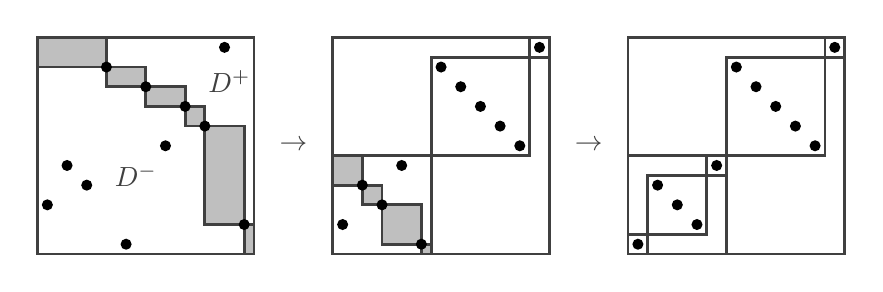
\begin{tikzpicture}[
	scale=0.25,
	baseline=(current bounding box.center),
	thickboxes
]
	\draw [draw=none, fill=white] (0,0) rectangle ++(42,12);
	
	\draw [fill=lightgray] (0.5,11.5) 
		|- (4,10)
		|- (6,9)
		|- (8,8)
		|- (9,7)
		|- (11,2)
		|- (11.5,0.5) 
		|- (11,2)
		|- (9,7)
		|- (8,8)
		|- (6,9)
		|- (4,10)
		|- cycle;
	\draw (0.5,0.5) rectangle ++(11,11);

	\foreach \y [count=\x] in {3, 5, 4, 10, 1, 9, 6, 8, 7, 11, 2} {
		\draw[myCircle] (\x,\y) circle (8pt);
	}
	
	\node at (5.5,4.5) {$D^-$};
	\node at (10.25,9.25) {$D^+$};

	\node at (13.5,6) {$\rightarrow$};

	\begin{scope}[shift={(15,0)}]
		\draw[fill=lightgray] (0.5,5.5) 
			|- (2,4)
			|- (3,3)
			|- (5,1)
			|- (5.5,0.5)
			|- (5,1)
			|- (3,3)
			|- (2,4)
			|- cycle;
		
		\draw (0.5,0.5) 
			rectangle ++(5,5)
			rectangle ++(5,5)
			rectangle ++(1,1)
			rectangle ++(-11,-11);
		
		\foreach \y [count=\x] in {2, 4, 3, 5, 1, 10, 9, 8, 7, 6, 11} {
			\draw[myCircle] (\x,\y) circle (8pt);
		}
	\end{scope}
	
	\node at (28.5,6) {$\rightarrow$};
	
	\begin{scope}[shift={(30,0)}]
		\draw (0.5,0.5) 
			rectangle ++(1,1)
			rectangle ++(3,3)
			rectangle ++(1,1)
			rectangle ++(5,5)
			rectangle ++(1,1)
			rectangle ++(-11,-11)
			rectangle ++(5,5);
		
		\foreach \y [count=\x] in {1, 4, 3, 2, 5, 10, 9, 8, 7, 6, 11} {
			\draw[myCircle] (\x,\y) circle (8pt);
		}
	\end{scope}
\end{tikzpicture}
\end{document}